% Specify the type of document
\documentclass[a4paper,12pt]{article}

% Load a number of useful packages
\usepackage{graphicx}
\usepackage{amsmath,amssymb,amsfonts,amsthm}
\usepackage{gensymb}
\usepackage[margin=1.0in]{geometry}
\usepackage[colorlinks=true]{hyperref}
\usepackage{cite}
\usepackage[caption=false,font=footnotesize]{subfig}
\usepackage[table]{xcolor}
\usepackage{biblatex}
\usepackage[utf8]{inputenc}
\usepackage{subfig}
\usepackage{textcomp}
\usepackage{amsmath}
\usepackage{float}
\usepackage[labelfont=bf]{caption}
\usepackage{setspace}
\usepackage{siunitx}
\sisetup{output-exponent-marker=\ensuremath{\mathrm{e}}}

\usepackage{titlesec}
\titleformat*{\section}{\large\bfseries}
\titleformat*{\subsection}{\normalsize\bfseries}
\titleformat*{\subsubsection}{\normalsize\bfseries}
\usepackage{indentfirst}

% \usepackage{fancyhdr} 
% \pagestyle{fancy}
% \fancyhf{}
% \fancyheadoffset{0cm}
% \renewcommand{\headrulewidth}{0pt} 
% \renewcommand{\footrulewidth}{0pt}
% \fancyhead[R]{\thepage}


\setlength{\parindent}{0.5in}
\addbibresource{references.bib}


% Two more packages that make it easy to show MATLAB code
\usepackage[T1]{fontenc}
\usepackage{mathptmx}
\usepackage[framed,numbered]{matlab-prettifier}
\lstset{
	style = Matlab-editor,
	basicstyle=\mlttfamily\small,
}

% Say where pictures (if any) will be placed
\graphicspath{{./pictures/}}

% Define title and author (date is auto-generated, unless you define it)
\renewcommand{\baselinestretch}{2}

% Start of document
\begin{document}

\begin{center}
    \Large\textbf{ECE 470: Project Update 2}
    \end{center}
    \hspace*{\fill} \normalsize{Team: Jeffery Zhou, Kenneth Tochihara, Charlie Ray} 
    \newline
    \hspace*{\fill} TA: Dhruv Mathur
    \newline
    \hspace*{\fill} Section: Monday 9AM
    \newline
    \hspace*{\fill} Team Name: GouBot
	\pagenumbering{arabic}
	\section{Brief Project Update}\label{introduction}

During this project update, the team has a goal of creating and integrating a differential drive robot with the existing UR3 robot provided. The team is able to investigate the URDF files of each part and successfully integrate the two in an xacro file. This integration posed a lot of the challenges for the team. We approached the problem by first converting the existing UR3 xacro file to an URDF file and then modified it by adding in the numerous parts from the cart such as wheels, chasis, etc. However, doing so requires extensive knowledge about making objects using URDF which we do not have enough experience of. The fix was therefore to modify the existing \lstinline!ur3_robot.urdf.xacro! file by adding the differential robot alongside with a fixed joint to the chassis of the robot. The robot can be shown in the figure below: 

\begin{figure}[H]
	\begin{center}
	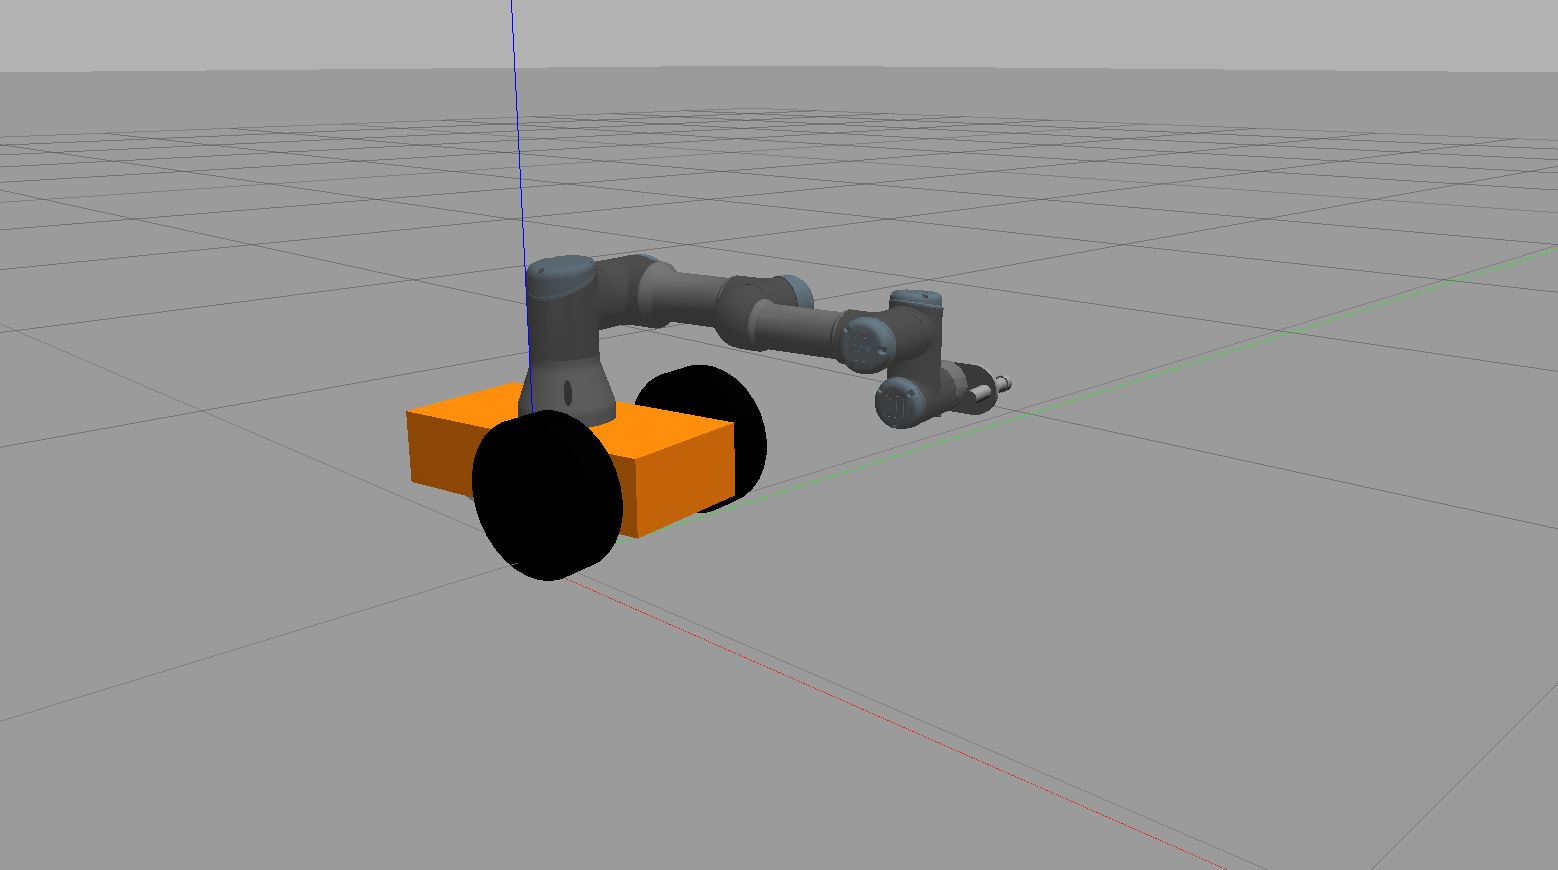
\includegraphics[width=0.7\columnwidth]{robot_with_arm.JPG}
	\caption{\textbf{Differential Robot with UR3 Attached}}
	\label{robot}
	\end{center}
\end{figure}

The next task was to make the entirety of the robotic structure move in a pre-determined pattern. However, the team could not make both the differential robot and the UR3 platform move. We then tested the code with the arms detached, the cart moved nicely in a circular pattern using \lstinline!circular_mode.py!. The team is now trying to fix the format of the current UR3 controller so that it could match that of athe UR3 driver. With that in mind, a \lstinline!.yaml! file needs to be made and integrated with the current robot controller. 


A successful testing in Gazebo using ROS can be seen in the YouTube video uploaded in the database on Github accessible using the link provided: \url{https://github.com/ktt3/ae482_goubot}.
\end{document}